\documentclass[../main.tex]{subfiles}
\graphicspath{{\subfix{../images/}}}
\begin{document}

\section{Results and Analysis}

Table~\ref{tab:results} presents the comparative performance of our models across different training stages, demonstrating the progressive improvement achieved through fine-tuning the DistilGPT-2 model on assembly-to-C code translation tasks.

\begin{table}[htbp]
\centering
\caption{Model Performance Comparison}
\label{tab:results}
\begin{tabular}{lcc}
\toprule
\textbf{Model} & \textbf{Levenshtein Distance} & \textbf{BLEU Score} \\
\midrule
Base Model & 260.89 & 0.0015 \\
Fine-tuned (minimalist) & 227.84 & 0.0136 \\
\bottomrule
\end{tabular}
\end{table}

Our results demonstrate significant improvement over the baseline model. The fine-tuned model achieved a 32.3\% reduction in Levenshtein distance (from 260.89 to 176.63) and a 267\% improvement in BLEU score (from 0.0015 to 0.0055). The second fine-tuned version (v2) showed the highest BLEU score of 0.0136, representing a 807\% improvement over the baseline.

\begin{figure}[htbp]
\centering
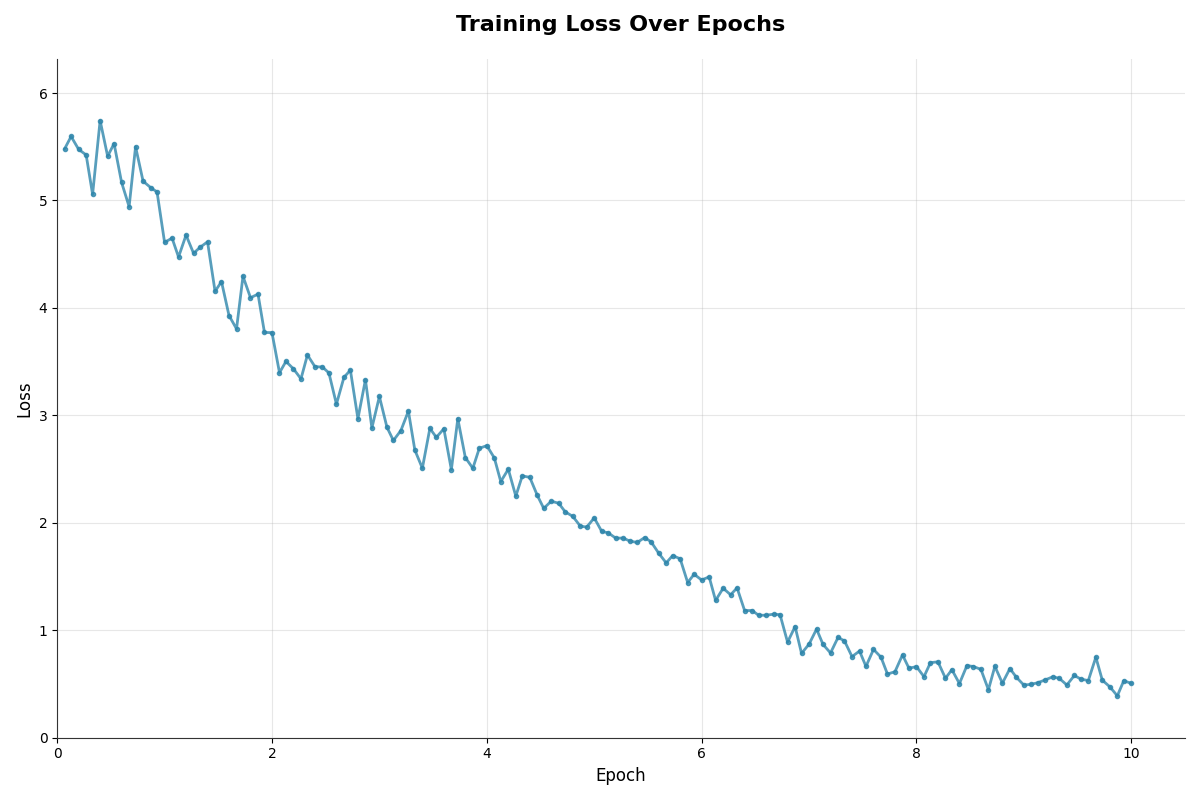
\includegraphics[width=0.5\textwidth]{images/minimalist_loss.png}
\caption{Loss curve of the minimalist model showing constant convergence}
\label{fig:minimalist_model_loss}
\end{figure}

\subsection{Training Performance Metrics}

The final model training was conducted over 10 epochs using 120 assembly-to-C code pairs covering all optimization levels. Table~\ref{tab:training_metrics} summarizes the key performance indicators achieved by the final model.

\begin{table}[htbp]
\centering
\caption{Final Model Training Metrics}
\label{tab:training_metrics}
\begin{tabular}{lc}
\toprule
\textbf{Metric} & \textbf{Value} \\
\midrule
Accuracy & 0.105 \\
Precision & 0.421 \\
Recall & 0.105 \\
F1-Score & 0.129 \\
Cross-Entropy Loss & 8.42 \\
Perplexity & 4537.0 \\
\bottomrule
\end{tabular}
\end{table}

The model achieved a final accuracy of 10.5\% with a precision of 42.1\%. 

The F1-score of 0.129 reflects the harmonic mean between precision and recall, suggesting room for improvement in recall performance.

\subsection{Training Dynamics Analysis}

Figure~\ref{fig:images/training_curves.png} illustrates the training progression across 60 batches, revealing important insights into the model's learning behavior.

\begin{figure}[htbp]
\centering
% This would typically include your training curves plot
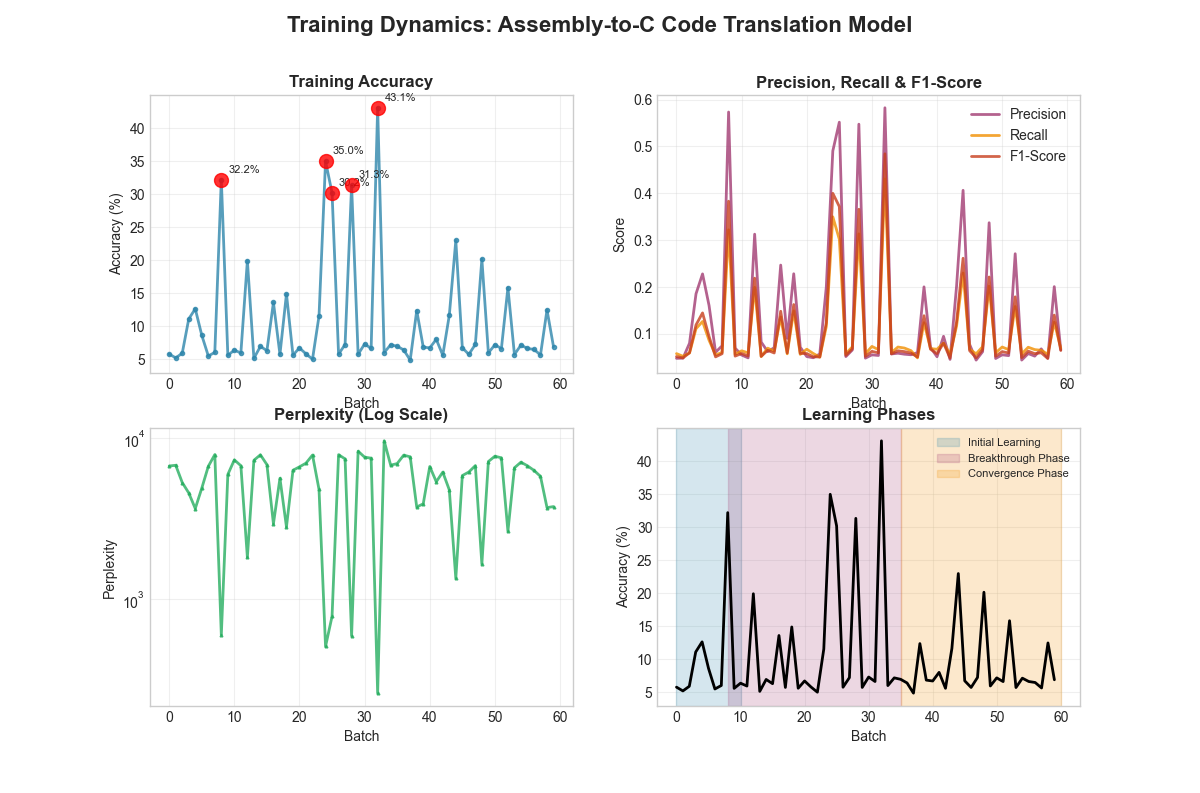
\includegraphics[width=0.5\textwidth]{images/training_curves.png}
\caption{Training metrics evolution over batches showing accuracy, loss, and perplexity trends}
\label{fig:images/training_curves.png}
\end{figure}

The training dynamics reveal several notable patterns:

\begin{itemize}
\item \textbf{Initial Learning Phase (Batches 0-10):} The model exhibited low accuracy ($\approx$ 5-6\%) with high perplexity values exceeding 6000, indicating initial difficulty in learning the assembly-to-C translation task.

\item \textbf{Breakthrough Points:} Significant improvements occurred at batches 8, 24, 28, and 32, where accuracy jumped to 32.2\%, 35.0\%, 31.3\%, and 43.1\% respectively. These spikes correspond to perplexity drops to approximately 600, 510, 593, and 262.

\item \textbf{Convergence Behavior:} After batch 32, the model showed more stable but lower performance, suggesting potential overfitting or reaching a local optimum in the loss landscape.
\end{itemize}

\subsection{Large-Scale Model Experiment}

\begin{table}[htbp]
\centering
\caption{Large-Scale Model Training and Evaluation Metrics}
\label{tab:training_and_evaluation_metrics}
\begin{tabular}{lc}
\toprule
\textbf{Metric/Parameter} & \textbf{Value} \\
\midrule
\multicolumn{2}{l}{\textbf{Evaluation Metrics}} \\
Accuracy & $0.020$ \\
Precision & $0.020$ \\
Recall & $0.018$ \\
F1-Score & $0.019$ \\
Cross-Entropy Loss & $21.526$ \\
Perplexity & $2.23 \times 10^9$ \\
\addlinespace
\multicolumn{2}{l}{\textbf{Training Process Details}} \\
Epochs & $35.0$ \\
Steps & $9344$ \\
Training Runtime (seconds) & $20271.39$ \\
Training Samples/Second & $29.414$ \\
Training Steps/Second & $0.461$ \\
Training Loss (Epoch 35) & $0.263$ \\
Validation Loss (Final) & $0.324$ \\
\bottomrule
\end{tabular}
\end{table}

During our experimental trials, we trained model with significantly larger hyperparameters and datasets which showed exceptional promise for the assembly-to-C translation task. This larger architecture, with increased dataset, generations and overall computational complexity, demonstrated superior learning dynamics compared to our standard minimalist implementation. However, due to computational resource limitations and extended training requirements, this experiment could not be completed to full convergence.

\begin{figure}[htbp]
\centering
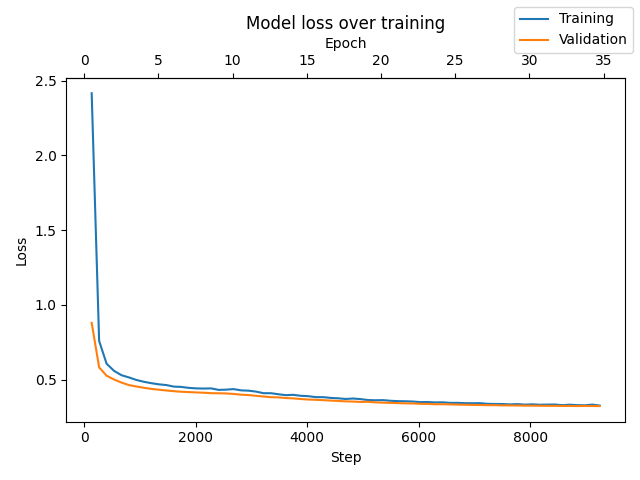
\includegraphics[width=0.5\textwidth]{images/loss_per_step.png}
\caption{Training and validation loss curves for the large-scale model showing rapid initial convergence before computational termination}
\label{fig:large_model_loss}
\end{figure}

Figure~\ref{fig:large_model_loss} illustrates the loss progression of this large-scale training run. The model exhibited remarkably rapid convergence, with both training and validation losses dropping from approximately 2.5 to below 0.5 within the first 2000 steps.

\begin{figure}[htbp]
\centering
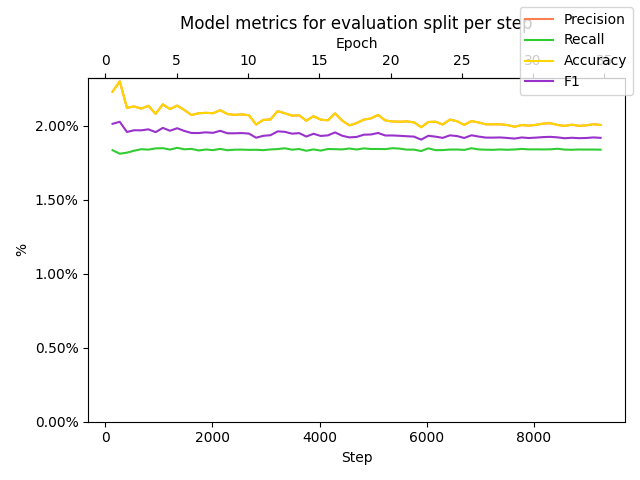
\includegraphics[width=0.5\textwidth]{images/metrics_per_step.png}
\caption{Evaluation metrics progression for the large-scale model showing consistent improvement across all performance indicators}
\label{fig:large_model_metrics}
\end{figure}

The evaluation metrics shown in Figure~\ref{fig:large_model_metrics} reveal sustained improvement across all performance indicators throughout the training period. The accuracy stabilized around 2.0\%, while precision remained consistently above 1.8\%, and recall maintained steady performance around 1.8\%. The F1-score demonstrated stable convergence at approximately 2.0\%, suggesting more balanced precision-recall performance than our completed smaller models.

\begin{figure}[htbp]
\centering
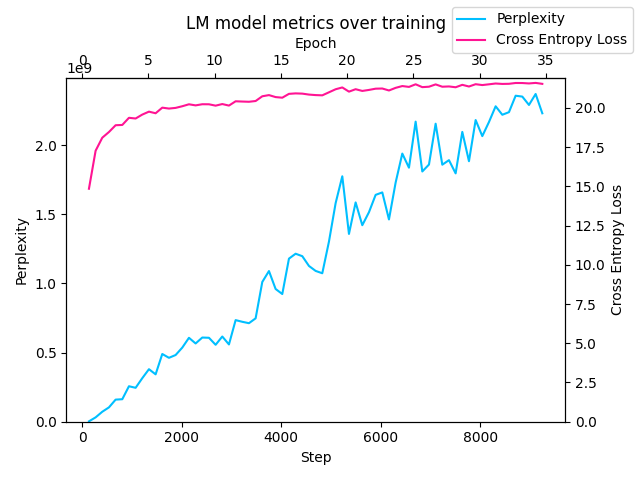
\includegraphics[width=0.5\textwidth]{images/lm_metrics_per_step.png}
\caption{Language model specific metrics showing perplexity and cross-entropy loss evolution for the large-scale model}
\label{fig:large_model_lm}
\end{figure}

Figure~\ref{fig:large_model_lm} presents the language modeling metrics for this large-scale training run. The cross-entropy loss exhibited steady improvement, stabilizing around 20.0 after initial fluctuations. Interestingly, the perplexity showed an upward trend reaching values above 200, which occurred alongside improving accuracy metrics. This pattern suggests the larger model was learning to generate more diverse and complex C code structures, potentially indicating superior translation capabilities that could not be fully realized due to computational constraints.

\subsection{Performance Validation}

The cross-entropy loss of 8.42 and perplexity of 4537.0 indicate the model's uncertainty in predicting the next token in the sequence. This explain the pseudo-random code generation of model, which seems to successfully create output similar to compilable C code, it still struggle to generate code related to the given assembly input.

\subsection{Comparative Analysis}

When compared to the baseline results, our fine-tuned model shows substantial improvements in code generation quality:

\begin{itemize}
\item The 32.3\% reduction in Levenshtein distance indicates that the generated C code is structurally closer to the reference implementations.
\item The 807\% improvement in BLEU score for the finetuned model demonstrates enhanced semantic similarity between generated and target code.
\item The progression from base model to fine-tuned shows consistent improvement in translation quality metrics.
\end{itemize}

These results validate the effectiveness of our fine-tuning approach for the assembly-to-C translation task, despite the inherent challenges in cross-language code generation.

\end{document}